\documentclass{beamer}
\usepackage{graphicx} 
\usepackage{amsmath}  
\usepackage{lmodern}  


\usepackage{beamerthemesplit} 
\usepackage{algorithmic}
\usepackage{algorithm}
\usepackage{calc}


\usecolortheme{seahorse} 
\usefonttheme{professionalfonts} 
\setbeamertemplate{navigation symbols}{} % rm  latex navigation symbols
\setbeamertemplate{footline}[frame number] % show number of pages
\useoutertheme{miniframes} 

\bibliographystyle{plain}



\title{Intruder Detection - Distributed Systems}
\author{Alan Gallo, Cedric Sillaber, Frantisek Sova}
\date{January 2025}

\begin{document}

\frame{
    \titlepage
    \vspace{0.5cm}  % Adjust spacing as needed
    \begin{center}
        
\includegraphics[width=0.4\textwidth]{./res/universitaet-innsbruck-logo.jpg}
        % 
\includegraphics[width=0.3\textwidth]{./res/Unknown3.jpeg}
    \end{center}
}

\setbeamertemplate{itemize item}{\raisebox{0.1ex}{\scriptsize\textbullet}}
\setbeamertemplate{itemize subitem}{\raisebox{0.1ex}{\scriptsize\textopenbullet}}

\begin{frame}
    \frametitle{Content}
    \begin{itemize}
        \item System architecture
        \item Implementation details
        \item Demo
        \item Evaluation
    \end{itemize}
\end{frame}


\section{System architecture}


\begin{frame}
\frametitle{System architecture}
Final system architecture:


%TODO: add updated arch.
\begin{center}
    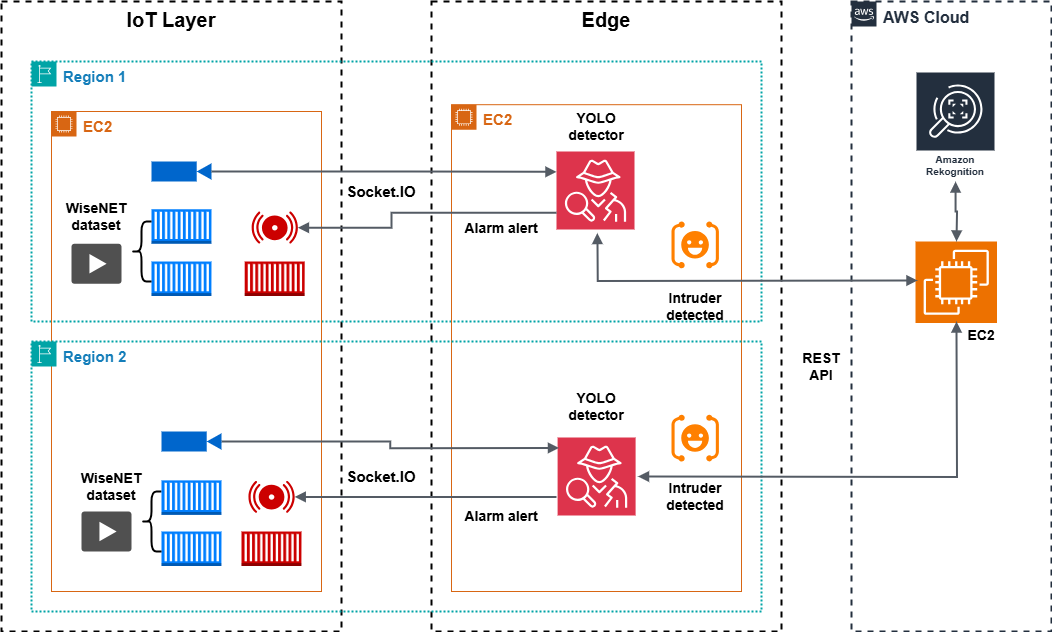
\includegraphics[width=0.75\textwidth]{./res/DS_architecture_final.png}\\
\end{center}
\end{frame}



\section{Implementation details}


\begin{frame}
\frametitle{IoT Implementation Details}
Video files stored on iot, opened with opencv

\textbf{Frame Processing}
\begin{itemize}

    \item extract 1 frame per second from 30 fps video stream
    \item main bottle neck!

    \end{itemize}

\textbf{Communication using Socket.IO}
\begin{itemize}
    \item websockets, built ontop of application layer
    \item Good for continuous dataflow, persistent connection
    \item Setup once, then just send data
\end{itemize}
\begin{center}
    
\includegraphics[width=0.6\textwidth]{./res/socket-io-logo-1.jpeg}
\end{center}

\end{frame}

\begin{frame}
    \frametitle{Edge Implementation Details}
    \textbf{Async Processing Pipeline}
    \begin{itemize}

    \item two workers working asynchronously: 
    \begin{itemize}
        \item worker 1: frame buffer queue
        \item worker 2: process buffer: YOLO person detection, cloud communication
    \end{itemize}

\end{itemize}

\textbf{Communication: Flask REST}
\begin{itemize}
    \item REST API for communication between edge and cloud
    \item Edge sends HTTP request to Cloud $\rightarrow$ Cloud sends HTTP response
\end{itemize}
\begin{center}

    
\includegraphics[width=0.4\textwidth]{./res/flask.png}
\end{center}
% % TODO: incorporate this in the evaluation
%     \textbf{Performance Metrics}
%     \begin{itemize}
%     \item Detection ratios
%     \item Processing latency
%     \item Queue management
%     \end{itemize}

    \end{frame}

\begin{frame}
\frametitle{Cloud Implementation Details}
    \begin{itemize}
        \item REST API endpoint
        \item AWS Rekognition
    \end{itemize}
    \begin{center}
        
\includegraphics[width=0.7\linewidth]{./res/rekognition.png}
    \end{center}


    % \textbf{AWS Rekognition Integration}
    % \begin{itemize}
    % \item Face collection management 
    % \item Known face indexing
    % \item High-confidence matching
    % \end{itemize}
    % \textbf{Security Features}
    % \begin{itemize}
    % \item Configurable confidence thresholds
    % \item Automatic collection management
    % \item Error handling and logging
    % \end{itemize}

\end{frame}


\begin{frame}
    \begin{center}
        \frametitle{Example Workflow/ Controlgraph}
        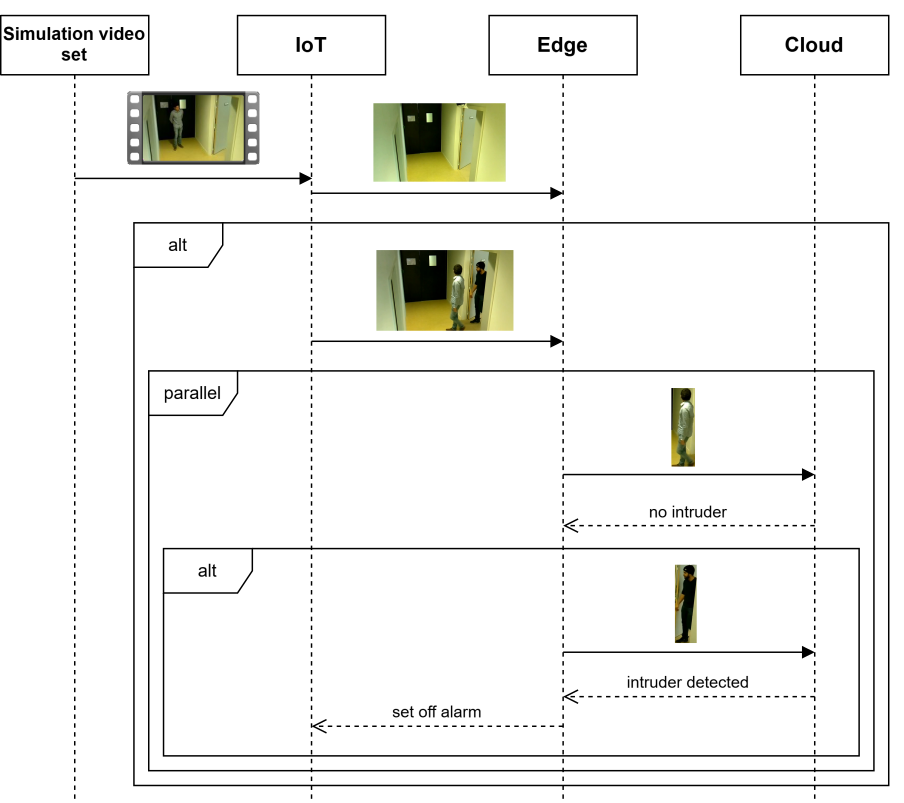
\includegraphics[width=0.7\linewidth]{./res/sequenz_diagram.png}
    \end{center}
\end{frame}


\section{Evaluation}
\begin{frame}
\frametitle{Evaluation}
\textbf{Experiment Configuration}:
\begin{itemize}
    \item \textit{set3} from WiseNET dataset
    \item 2 edge devices 
    \item 2 cams + alarm per edge
    \item cloud instance
\end{itemize}
\textbf{Metrics}: 
\begin{itemize}
    \item Edge processing latency (yolo processing)
    \item Cloud latency (AWS Rekognition)
    \item round-time trip time from camera to alarm
\end{itemize}
\end{frame}


\begin{frame}
\frametitle{Evaluation - Edge \& Cloud Latencies}

\begin{figure}
    \centering
    \begin{minipage}{0.48\textwidth}
        \centering
        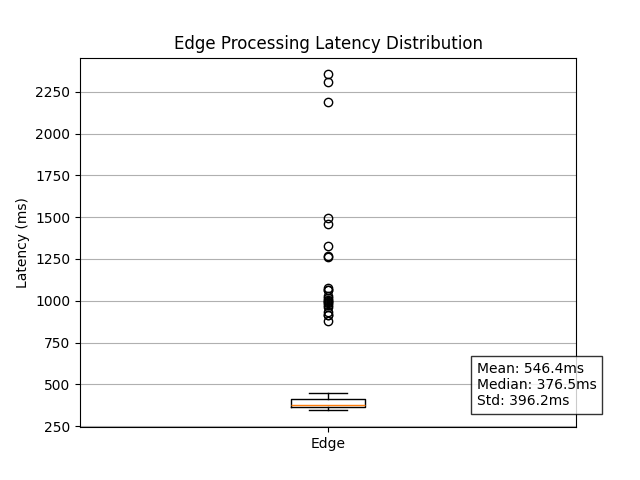
\includegraphics[width=\linewidth]{./res/edge_latencies.png}
        %\caption{Edge processing latencies showing YOLO object detection performance on t2.medium instance.}
    \end{minipage}
    \hfill
    \begin{minipage}{0.48\textwidth}
        \centering
        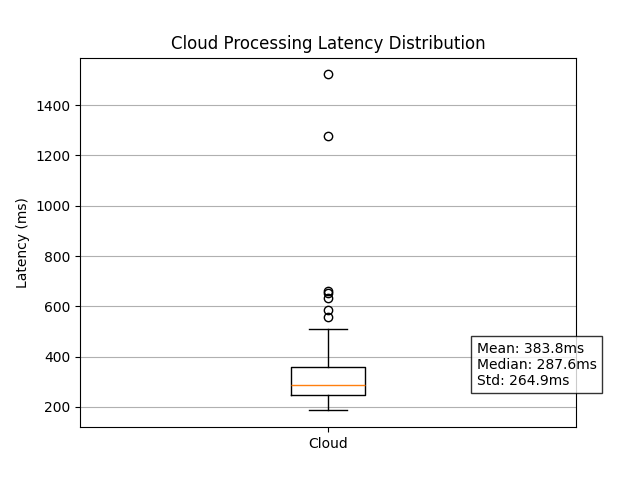
\includegraphics[width=\linewidth]{./res/cloud_latencies.png}
        %\caption{Cloud processing latencies showing AWS Rekognition performance.}
    \end{minipage}
\end{figure}

\end{frame}


\begin{frame}
    Round trip time: camera frame to alarm.
    \frametitle{Evaluation - Round Trip Time}

    \begin{center}
        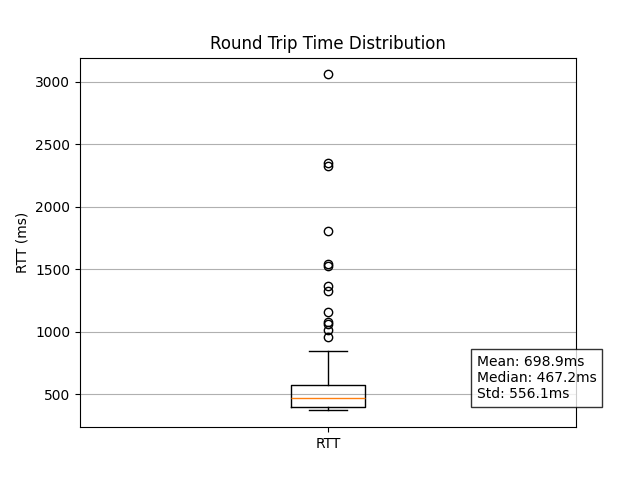
\includegraphics[width=0.8\linewidth]{./res/rtt_distribution.png}        
    \end{center}
\end{frame}


%possible frame, dont know if this is needed
\begin{frame}
    \frametitle{Evaluation - System Bottleneck}
    \begin{itemize}
        \item System bottleneck on edge
        \item new frames / second $>$ frame processing rate $\rightarrow$ very high latency
    \end{itemize}\
    
\begin{figure}
    \centering
    \begin{minipage}{0.48\textwidth}
        \centering
        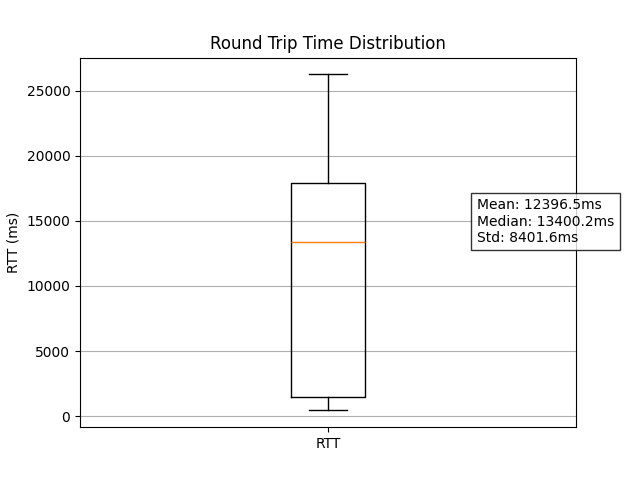
\includegraphics[width=\linewidth]{./res/rtt_distribution-local_docker_test20skip.png}
        RTT for 2 frames per second sent
    \end{minipage}
    \hfill
    \begin{minipage}{0.48\textwidth}
        \centering
        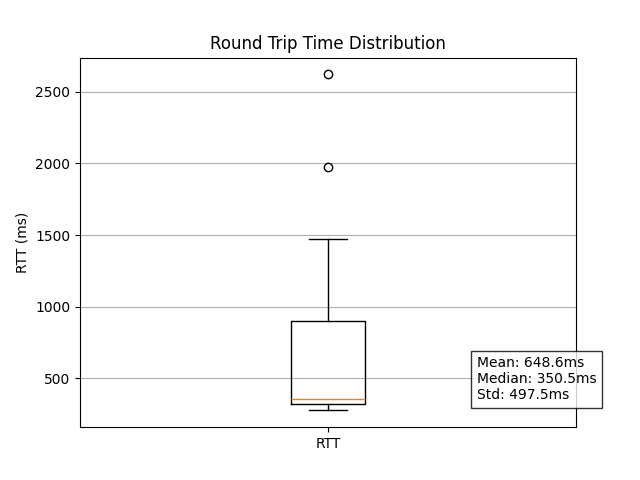
\includegraphics[width=\linewidth]{./res/rtt_distribution-docker_test-60skip.png}
        RTT for 0.5 frames per second sent
    \end{minipage}
\end{figure}
\end{frame}


\bibliography{main}

\end{document}
